\chapter{Used Technologies}
\label{chapter:AutoTechnologies}

In addition to the technologies used in the first part of this
thesis (see Chapter \ref{chapter:ConfTechnology}) other Eclipse
technologies will be used as well.

The next sections will describe the technologies and give some
examples of their usage in the standard Eclipse application.
The technologies described here are the following:
\begin{description}
 \item The Job: The Eclipse Job is a mechanism for very long running tasks.
 \item The Wizard: The wizard is a method for helping the user to set up complex tasks.
\end{description}


\section{The Job}
\label{section:AutoTechJob}

The Eclipse Job \ac{API} provides the means to schedule very long running tasks.
It uses a Thread to run the actual task and contains a ProgressMonitor to show
the progress of the task. Since it is a task that can run independently of the
current state of the workspace it can also be run in the back ground if the user
desires it.
An example for the use of jobs in the normal Eclipse architecture
is the SVN commit operation seen in Figure \ref{fig:SVNCommit}.

\begin{figure}[SVNCommit]
  \centering
  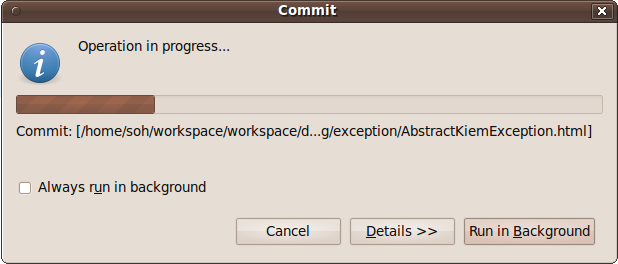
\includegraphics[scale=.4]{SVNCommit.png}
  \caption[The SVN commit job]%
  {The SVN commit job\protect}
  \label{fig:SVNCommit}
\end{figure}

\section{Eclipse Wizards}
\label{section:AutoTechWizards}
\index{Wizard}
Wizards are used to guide the user through the process of creating complex items by taking
the information in a structured way and then generating the item from it. A wizard is 
basically a multi-page dialog with each page representing one step in the creation of the 
desired item.

One example inside the Eclipse Architecture is the Java Class Creation Wizard (see Figure \ref{fig:ClassWizard})
In theory it is possible to open a text file and enter all the information manually.
However if the wizard is used the user only has to select the class he wants to extend
and the interfaces he wants to implement, activate one check box and then the wizard will
create the class body, all required methods and comments for each element (see Listing \ref{list:classCreationGenerated})
This makes it very easy for even inexperienced users to create new classes without knowing
the exact syntax.

\begin{figure}[ClassWizard]
  \centering
  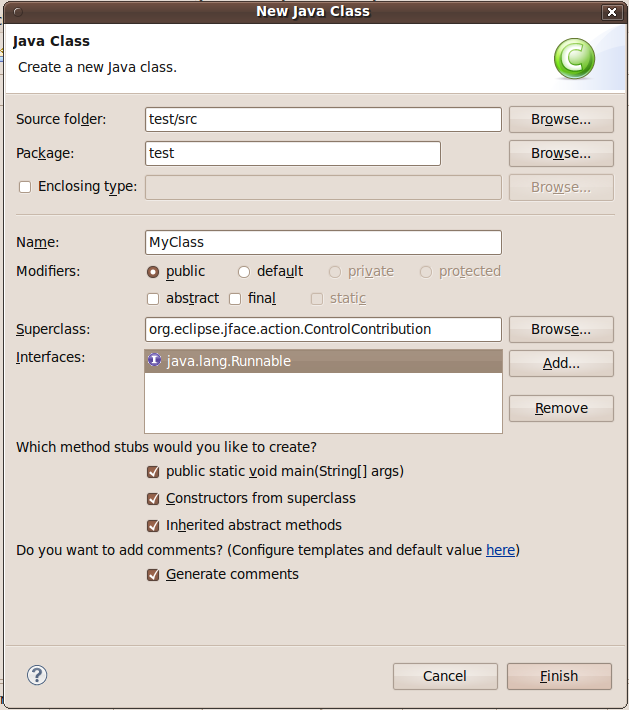
\includegraphics[scale=.4]{ClassWizard.png}
  \caption[The Class Creation Wizard]%
  {The Class Creation Wizard\protect}
  \label{fig:ClassWizard}
\end{figure}

\listingjava
\showlistingex{code/newClassGenerated.txt}
{Java}
{Code generated by the wizard}
{list:classCreationGenerated}
{t}

